\documentclass{article}
\usepackage{amsmath}
\usepackage{mathtools}
\usepackage{amssymb}
\usepackage{listings}
\usepackage{xcolor}
\usepackage{geometry}
\usepackage{titlesec}
\setlength{\parindent}{0pt}
\setlength{\parskip}{0.5em}
\usepackage{graphicx}
\usepackage{float}
\setlength{\parskip}{0.5em}
\setlength{\parindent}{0pt}
\usepackage{placeins}
\renewcommand{\thesubsection}{\thesection.\arabic{subsection}}

% Define colors
\definecolor{codegreen}{rgb}{0,0.6,0}
\definecolor{codegray}{rgb}{0.5,0.5,0.5}
\definecolor{codepurple}{rgb}{0.58,0,0.82}
\definecolor{backcolour}{rgb}{0.95,0.95,0.92}
\definecolor{keywordcolor}{rgb}{0.5,0,0.5}
\definecolor{stringcolor}{rgb}{0.25,0.5,0.35}
\definecolor{commentcolor}{rgb}{0.25,0.35,0.75}
\definecolor{numbercolor}{rgb}{0.7,0.7,0.7}

% Setup the listings package
\lstdefinestyle{mystyle}{
    backgroundcolor=\color{backcolour},   
    commentstyle=\color{commentcolor},
    keywordstyle=\color{keywordcolor},
    numberstyle=\tiny\color{numbercolor},
    stringstyle=\color{stringcolor},
    basicstyle=\ttfamily\footnotesize,
    breakatwhitespace=false,         
    breaklines=true,                 
    captionpos=b,                    
    keepspaces=true,                 
    numbers=left,                    
    numbersep=5pt,                  
    showspaces=false,                
    showstringspaces=false,
    showtabs=false,                  
    tabsize=2
}

\lstset{style=mystyle, language=Java}

% Adjust margins
\geometry{
  left=1in,
  right=1in,
  top=1.0in,
  bottom=1.5in,
  headheight=0ex,
  headsep=0ex,
  footskip=0.5in
}

\newcommand{\designpattern}[1]{\textbf{\textit{\textcolor{purple}{#1}}}}
\newcommand{\designclass}[1]{\textit{\textcolor{brown}{#1}}}
\newcommand{\application}[1]{\textbf{\textcolor{codegreen}{#1}}}

% Adjust title spacing: left, before, after
\titleformat*{\section}{\large\bfseries}
\titlespacing*{\section}{0pt}{*1.0}{*1.0}

\title{Final Project MPCS 51050 - Event Market}
\author{Fernando Rocha Urbano}
\date{April 2024}

% Define colors
\definecolor{codegreen}{rgb}{0,0.6,0}
\definecolor{codegray}{rgb}{0.5,0.5,0.5}
\definecolor{codepurple}{rgb}{0.58,0,0.82}
\definecolor{backcolour}{rgb}{0.95,0.95,0.92}

% Setup the listings package
\lstdefinestyle{mystyle}{
    backgroundcolor=\color{backcolour},   
    commentstyle=\color{codegreen},
    keywordstyle=\color{magenta},
    numberstyle=\tiny\color{codegray},
    stringstyle=\color{codepurple},
    basicstyle=\ttfamily\footnotesize,
    breakatwhitespace=false,         
    breaklines=true,                 
    captionpos=b,                    
    keepspaces=true,                 
    numbers=left,                    
    numbersep=5pt,                  
    showspaces=false,                
    showstringspaces=false,
    showtabs=false,                  
    tabsize=2
}

\lstset{style=mystyle}

\begin{document}

\maketitle

\FloatBarrier
\section{General Topic}
We aim to build an Event Ticket Purchase Platform, including event creation, purchase app, notification system, payment validation, event recommender engine.

In order to facilitate the understanding we highlight the following with specific formatting:
\begin{itemize}
    \item \application{Application Names}
    \item \designpattern{Design Patterns}
    \item \designclass{Classes}
\end{itemize}

\FloatBarrier
\section{Project Separation}
\FloatBarrier
\subsection{Creation Processes}
\begin{figure}[h]
    \centering
    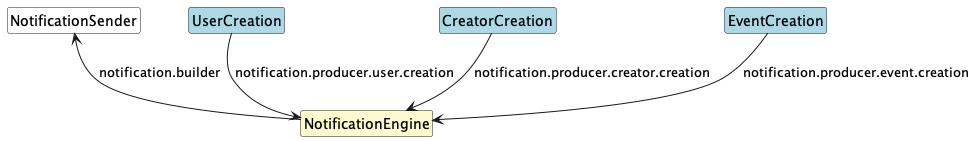
\includegraphics[width=\textwidth, height=350px, keepaspectratio]{assets/uml/structure/Creation.png}
\end{figure}

\FloatBarrier
\subsection{Ticket Purchase Processes}
\begin{figure}[h]
    \centering
    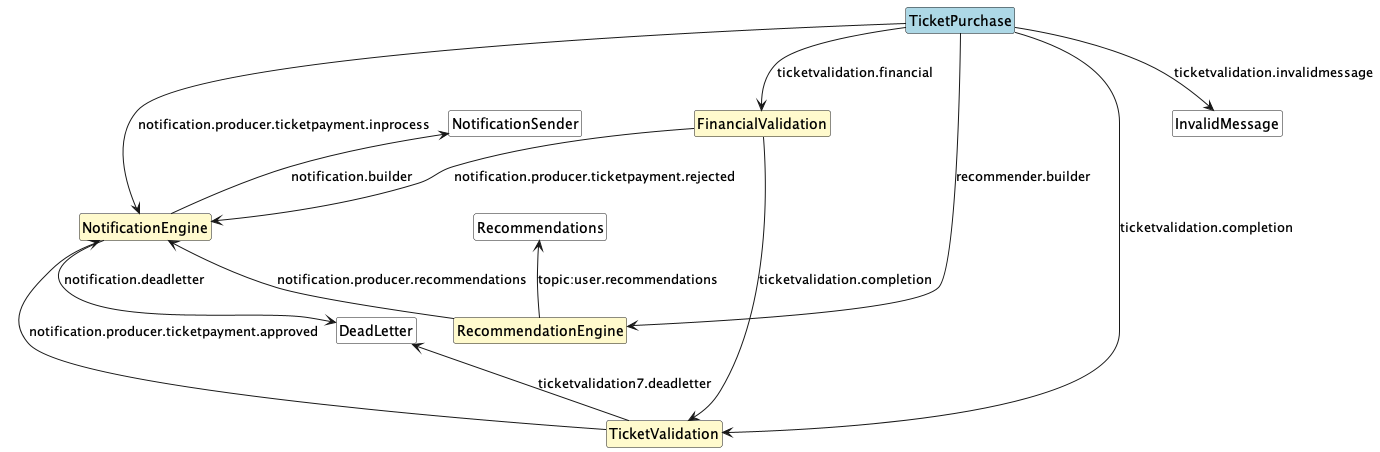
\includegraphics[width=\textwidth, height=350px, keepaspectratio]{assets/uml/structure/Purchase.png}
\end{figure}

\FloatBarrier
\section{Applications}
\begin{itemize}
    \item Main Application with Database connection:
    \begin{itemize}
        \item \application{Event Market: event-market}
    \end{itemize}
    \item Creation Camel Applications:
    \begin{itemize}
        \item \application{Event Creation: event-market-event-creation}
        \item \application{User Creation: event-market-user-creation}
        \item \application{Creator Creation: event-market-event-creation}
    \end{itemize}
    \item Ticket Purchase Camel Applications:
    \begin{itemize}
        \item \application{Ticket Purchase: event-market-ticket-purchase}
        \item \application{Financial Validation: event-market-financial-validation}
        \item \application{Ticket Validation: event-market-ticket-validation}
        \item \application{Event Recommender Engine: event-market-recommendation-engine}
        \item \application{Notification Engine: event-market-notification-engine}
    \end{itemize}
\end{itemize}

\FloatBarrier
\section{Design Patterns}
\FloatBarrier
\subsection{Iterator}
\begin{itemize}
    \item Inside the \application{Ticket Purchase} app.
    \item Iterator pattern is used inside the \designclass{TicketTypeIterator} class to iterate over the ticket types of an Event.
    \item Provides a convenient way for users to browse through various ticket options, helping them understand the minimum age, prices, and types of tickets available for an event.
\end{itemize}

\FloatBarrier
\subsection{Singleton}
\begin{itemize}
\item Inside the \application{Financial Validation} app.
\item The \designclass{FinancialValidator} class is a Singleton, ensuring that a single instance validates ticket requests and manages their statuses.
\item The Singleton pattern allows the \designclass{FinancialValidator} to track which requests it has validated recently, avoiding redundant checks and improving efficiency.
\end{itemize}

\FloatBarrier
\subsection{Strategy}
\begin{itemize}
\item Inside the \application{Financial Validation} app.
\item The \designclass{PaymentMethod} class acts as a Strategy pattern, providing an interface implemented by different payment classes such as \designclass{CheckingsAccountPayment} and \designclass{CardPayment}.
\item This pattern enables the \designclass{Financial Validation} app to support various payment methods flexibly, facilitating future additions or modifications by simply extending the interface.
\end{itemize}

\FloatBarrier
\subsection{Facade}
\begin{itemize}
\item Inside the \application{Event Recommender Engine}.
\item The \designclass{EventRecommender} class acts as a Facade, simplifying the complexity of underlying classes derived from the \designclass{AbstractRecommenderModel}.
\item This pattern allows for interactions with different recommendation models, making it easier to generate recommendations for users based on recent ticket requests.
\end{itemize}

\FloatBarrier
\subsection{Template Method}
\begin{itemize}
\item Inside the \application{Event Recommender Engine}.
\item The Template Method pattern is used by \designclass{AbstractRecommenderModel} and its derived classes, implementing some functionalities while leaving the heavy lifting to derived classes.
\item This pattern provides a clear structure for creating different recommendation models, allowing derived classes to implement the specific logic needed to generate suggestions for users.
\end{itemize}

\FloatBarrier
\section{Applications and UML Drawings}
\FloatBarrier
\subsection{Event Creation}
App creates a new instances of \designclass{Event}.

The \designclass{Event} class has:
\begin{itemize}
    \item at least one \designclass{TicketType} instance: for instance, premium, normal, free, etc... which specifies the price, minimum age, total tickets for the type.
    \item one \designclass{Location} instance.
    \item one \designclass{Creator} (each \designclass{Creator} can have multiple events).
\end{itemize}

\begin{figure}[h]
    \centering
    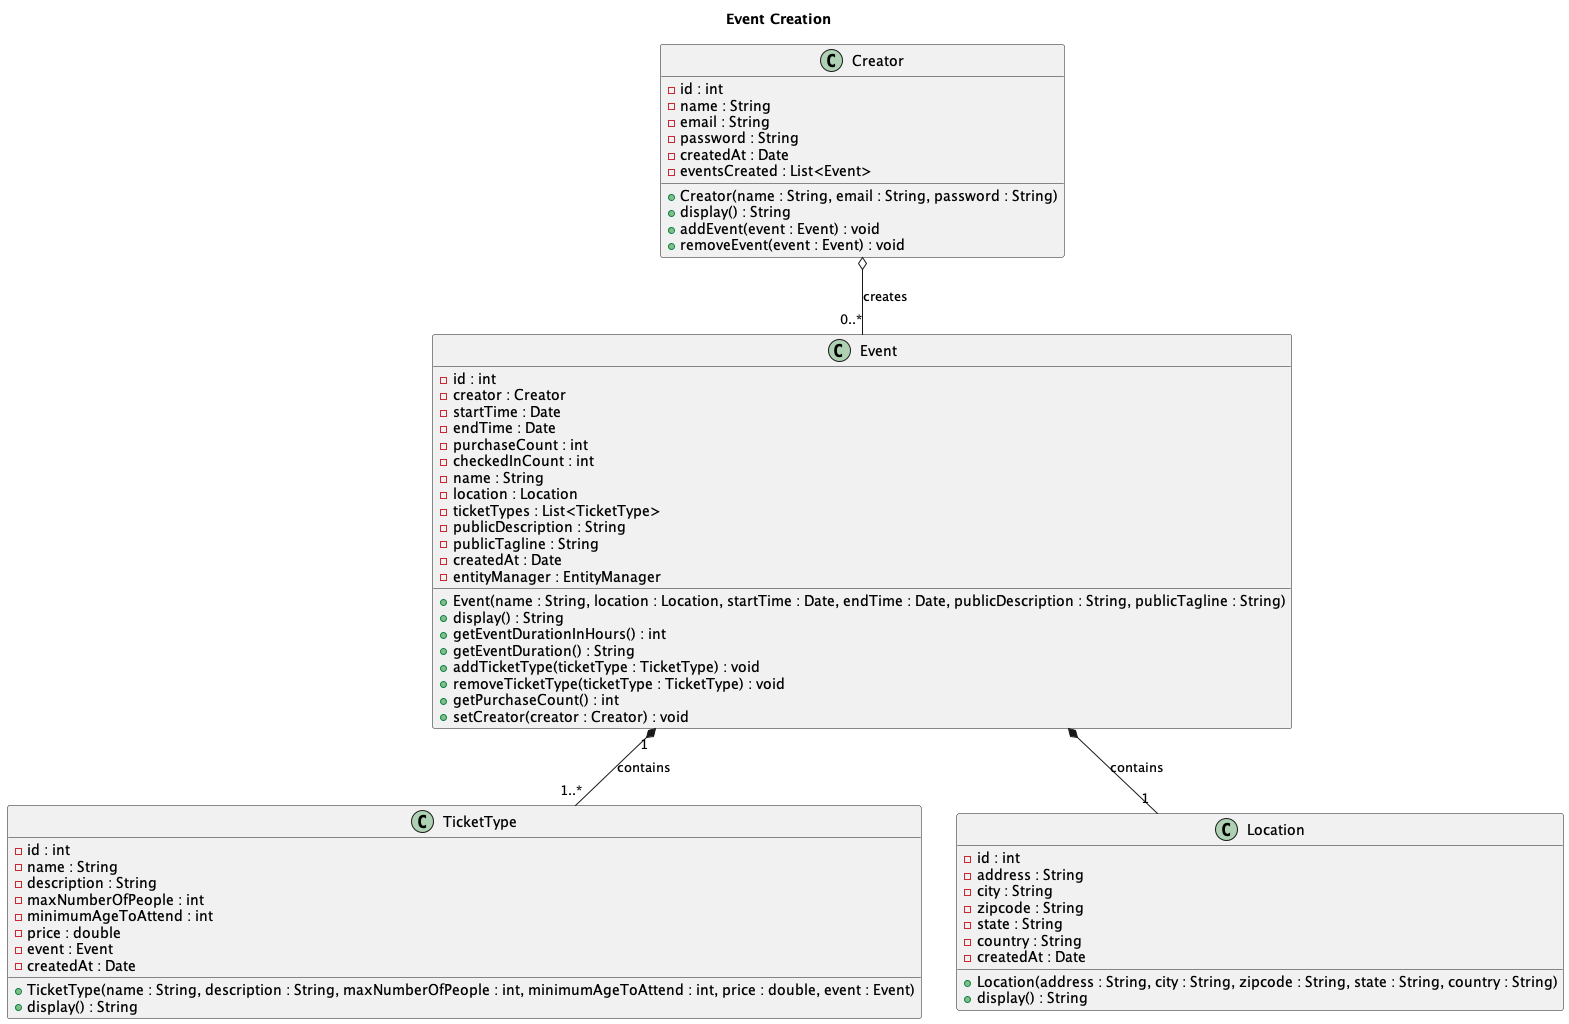
\includegraphics[width=\textwidth, height=350px, keepaspectratio]{assets/uml/relations/EventCreation.png}
\end{figure}

THe application communicates with \application{Notification Engine}.

\subsection{User Creation}
Similar to the creation of Event. THe application communicates with \application{Notification Engine}.

\subsection{Creator Creation}
Similar to the creation of Event. THe application communicates with \application{Notification Engine}.

\FloatBarrier
\subsection{Ticket Purchase}
App allows purchase of tickets from \designclass{User}.

The \designclass{TicketRequest} is the main class in this process.

Every \designclass{TicketRequest} instance has an instance of:
\begin{itemize}
    \item \designclass{TicketType}: the type of ticket the user is buying. A single event allows for multiple \designclass{TicketType}'s with different prices, descriptions, etc. A \designclass{TicketRequest} instance only has one \designclass{TicketType} instance among the ones available for the event.
    \item \designclass{Financial Information}: the information regarding the payment of the ticket. Each instance of it has one instance of a class derived from \designclass{PaymentMethod}, which can be \designclass{CheckingsAccountPayment} or \designclass{CardPayment}. In case the ticket price is 0, the \designclass{FinancialInformation} is not necessary.
    \item \designclass{User}: the person purchasing the ticket.
    \item \designclass{Recipient}: the person who will enter the event. An instance of class \designclass{User} can be transformed into an instance of the class \designclass{Recipient} in case the user is trying to buy a ticket for himself/herself.
\end{itemize}

Once the \designclass{TicketRequest} is completed, it is sent to:
\begin{itemize}
    \item the \application{Financial Validation} in case a payment is necessary.
    \item the \application{Ticket Validation} in case no payment is necessary.
    \item the \application{Event Recommender Engine} regardless of payment options.
    \item the \application{Notification Engine} to say that the ticket is being processed.
\end{itemize}

Inside the \application{Ticket Purchase} we use the \designpattern{Iterator} pattern with \designclass{TicketTypeIterator}, which receives an \designclass{Event} and iterates over the ticket types. The iterator is considerably useful for the \designclass{User} to understand the minimum age among all the ticket types, the minimum and maximum price of the event, etc...

\begin{figure}[h]
    \centering
    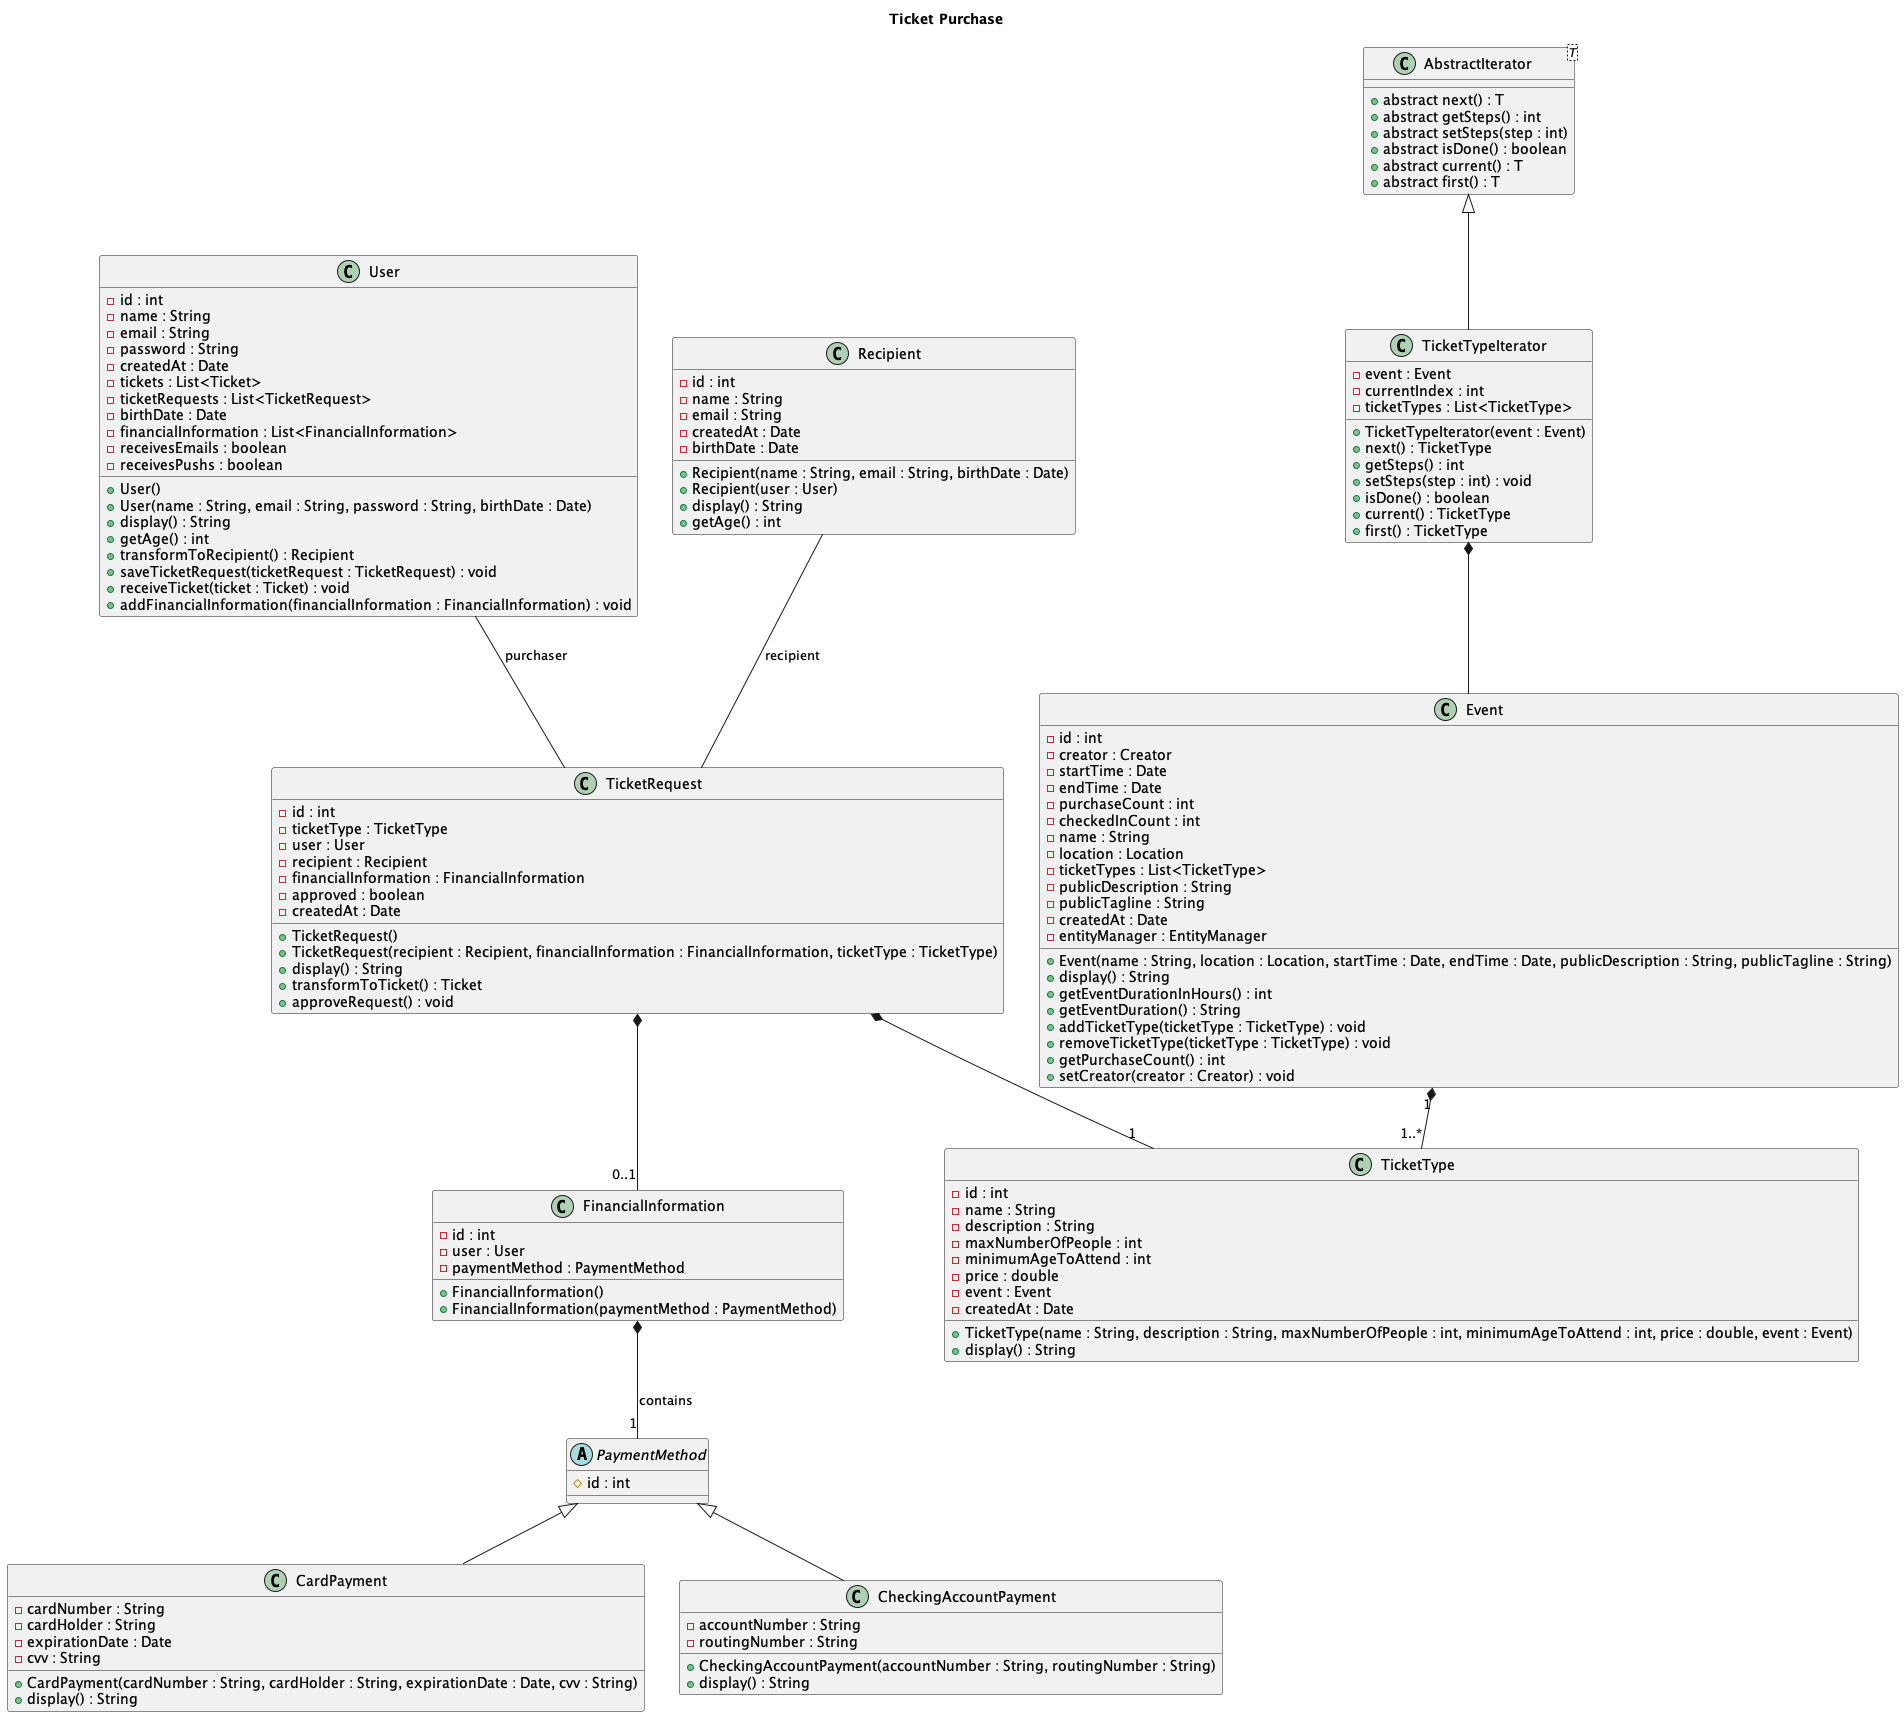
\includegraphics[width=\textwidth, keepaspectratio]{assets/uml/relations/TicketPurchase.png}
\end{figure}

\FloatBarrier
\subsection{Financial Validation}
App gets messages from the distributed message queue saying that a \designclass{TicketRequest} needs payment validation.

Inside the app, The \designclass{TicketRequest} is sent to the \designclass{FinancialValidator} which ask for a payment process.

The \designclass{FinancialValidator} is a \designpattern{Singleton} because it aims to track which instances of \designclass{TicketRequest} it has checked recently: this allows the \designclass{FinancialValidator} to avoid wasting time checking twice the same \designclass{TicketRequest}.

The \designclass{TicketRequest} instance has an instance of \designclass{FinancialInformation}, which has one instance of a class derived from \designclass{PaymentMethod}.

The available classes are:
\begin{itemize}
    \item \designclass{CardPayment}
    \item \designclass{CheckingsAccountPayment}
\end{itemize}

\designclass{PaymentMethod} is a \designpattern{Strategy} pattern.

The \designclass{FinancialValidator} must be able to handle both classes.

Therefore, if there is an addition/change in those classes, the \designclass{FinancialValidator} must be changed/incremented as well.

Finally, the \designclass{FinancialValidator} sends a request to the desired bank to approve the payment (here we simplified the implementation and just randomly approve or reject the payment).

The application sends message to the 
\begin{itemize}
    \item the \application{Ticket Validation} in case the payment is accepted.
    \item the \application{Notification Engine} in case the payment is rejected.
\end{itemize}

\begin{figure}[h]
    \centering
    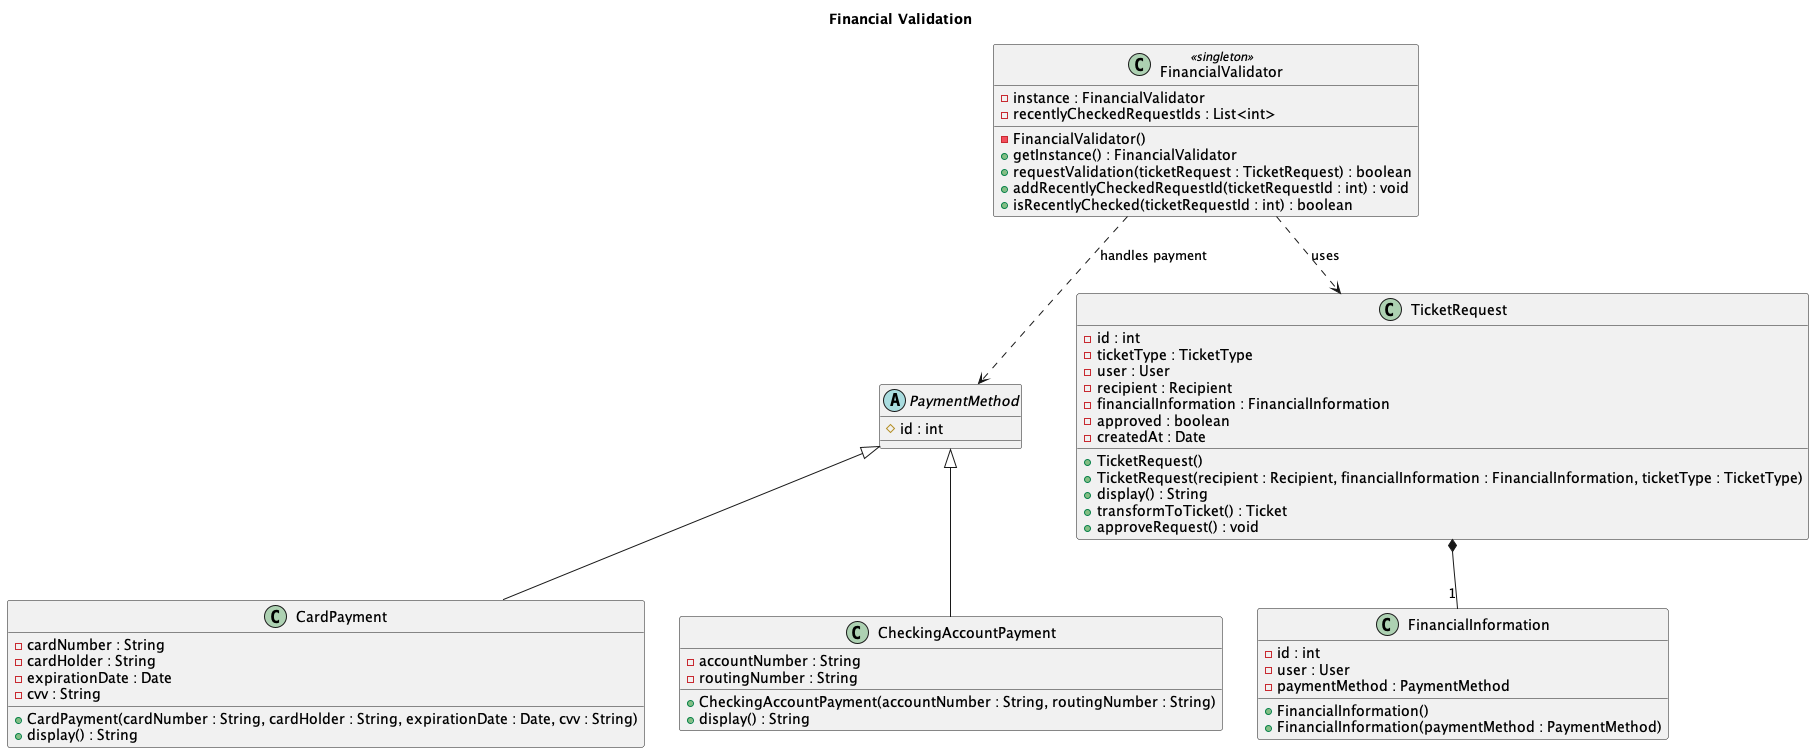
\includegraphics[width=\textwidth, height=350px, keepaspectratio]{assets/uml/relations/FinancialValidation.png}
\end{figure}

\FloatBarrier
\subsection{Ticket Validation}
App gets messages from the distributed message queue saying that the ticket for that \designclass{User} has been approved.

The \designclass{Ticket} instance is created with a \designclass{TicketRequest} instance inside. The \designclass{TicketRequest} contains all the information about the \designclass{Event} inside it.

The \designclass{Ticket} instance is added to the \designclass{User}. More specifically, the \designclass{Ticket} instance is added to a list of owned tickets and remove the instance of \designclass{TicketRequest} from the list of requested tickets.

Finally, a message is sent to the \application{Notification Engine}.

\begin{figure}[h]
    \centering
    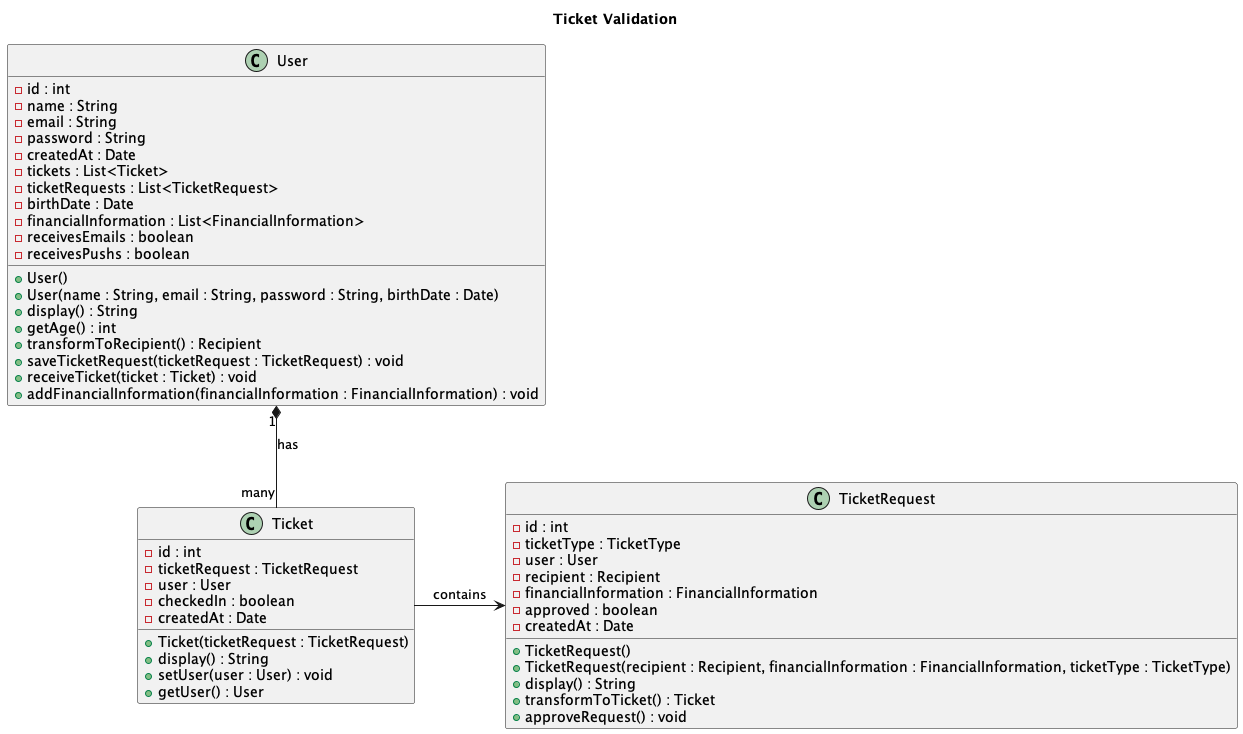
\includegraphics[width=\textwidth, height=350px, keepaspectratio]{assets/uml/relations/TicketValidation.png}
\end{figure}

\FloatBarrier
\subsection{Event Recommender Engine}
App creates recommendations to the \designclass{User} based on recent purchases.

The event recommender engine receives a message everytime a \designclass{User} uses the \application{Ticket Purchase} application.

The \designclass{EventRecommender} class takes \designclass{User} and a model name (the one that is currently being used) and creates a recommendation for the user based on recent ticket requests.

The \designclass{EventRecommender} works as a \designpattern{Facade} as it simplifies the underlying complexity of classes derived from the \designclass{AbstractRecommenderModel}, like \designclass{NlpRecommenderModel} and \designclass{PopularityRecommenderModel}.

We have a \designpattern{Template Method} with the \designclass{AbstractRecommenderModel} and its derived classes. The \designclass{AbstractRecommenderModel} implements some of the functionalities of the model, but leaves the heavy lifting of creating suggestions for the derived classes.

It sends messages to the \application{Notification Engine}.

\begin{figure}[h]
    \centering
    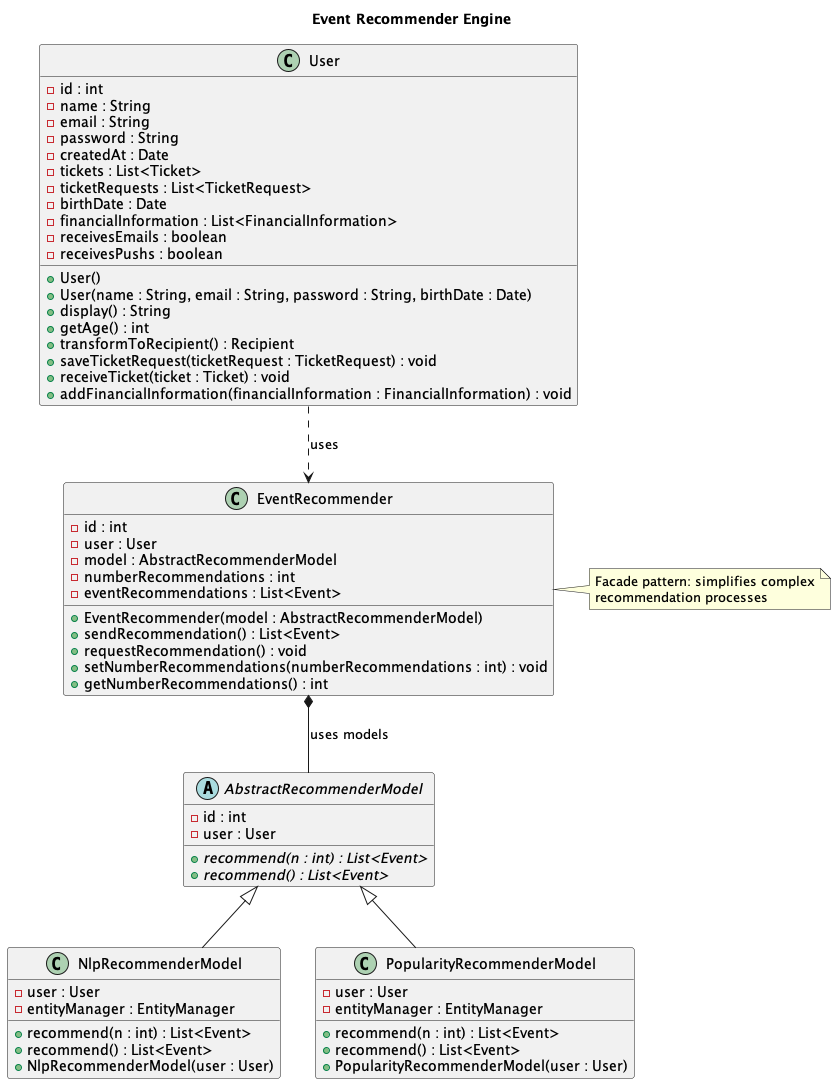
\includegraphics[width=\textwidth, height=350px, keepaspectratio]{assets/uml/relations/EventRecommenderEngine.png}
\end{figure}

\FloatBarrier
\subsection{Notification Engine}
The app translates internal information of the system into proper notifications for the users, allowing the market department to modify the content to better address the \designclass{User} or \designclass{Creator}.

It sends message to the Notification Sender (which could later just send the notification to the user or creator.)

\FloatBarrier
\section{EIP Patterns}

\begin{enumerate}
    \item \textbf{Message Channel and Endpoint:} How we connect an application to the channel. It is used in every single application.
    \item \textbf{Content-Based Router:} Routes each message to the correct recipient based on message content.
    \item \textbf{Dead-Letter Channel:} The messaging system determines that it cannot or should not deliver a message. It is used (in our case and generally) for messages that cannot be processed successfully after a certain amount of tries.
    \item \textbf{Invalid-Message Channel:} Channel for messages that are malformed or fail validation checks and cannot be processed as expected.
    \item \textbf{Message Translator:} Used between other filters or applications to translate one data format into another.
    \item \textbf{Wire Tap:} Inserts a simple Recipient List into the channel that publishes each incoming message to the main channel and a secondary channel.
    \item \textbf{Normalizer:} Routes each message type through a custom Message Translator so that the resulting messages match a common format.
    \item \textbf{Content Enricher:} Access an external data source in order to augment a message with missing information.
    \item \textbf{Multicast:} Allows a message to be sent to multiple recipients or destinations simultaneously (not in the book, but included in Camel: https://camel.apache.org/components/4.4.x/eips/multicast-eip.html).
\end{enumerate}

\FloatBarrier
\subsection{Event-Market Applications}

\subsection{event-market-user-creation: User Creation Producer}
\begin{enumerate}
    \item \textbf{Message Channel}
\begin{lstlisting}[language=Java, caption={Message Channel for User Creation}]
to("jms:queue:notification.producer.user.creation.queue")
\end{lstlisting}
    \item \textbf{Point-to-Point Channel:} Inherited and implemented by this type of queue.
\end{enumerate}

\subsection{event-market-creator-creation: Creator Creation Producer}
\begin{enumerate}
    \item \textbf{Message Channel}
\begin{lstlisting}[language=Java, caption={Message Channel for Creator Creation}]
to("jms:queue:notification.producer.creator.creation.queue")
\end{lstlisting}
    \item \textbf{Point-to-Point Channel:} Inherited and implemented by this type of queue.
\end{enumerate}

\subsection{event-market-event-creation: Event Creation Producer}
\begin{enumerate}
    \item \textbf{Message Channel}
\begin{lstlisting}[language=Java, caption={Message Channel for Event Creation}]
to("jms:queue:notification.producer.event.creation.queue")
\end{lstlisting}
    \item \textbf{Point-to-Point Channel:} Inherited and implemented by this type of queue.
\end{enumerate}

\subsection{event-market-notification-engine: Notification Engine Producer}
\begin{enumerate}
    \item \textbf{Message Channel}
\begin{lstlisting}[language=Java, caption={Message Channels for Notification Engine}]
from("jms:queue:notification.producer.user.creation.queue")
from("jms:queue:notification.producer.creator.creation.queue")
from("jms:queue:notification.producer.event.creation.queue")
from("jms:queue:notification.producer.ticketpayment.inprocess.queue")
from("jms:queue:notification.producer.ticketpayment.rejected.queue")
from("jms:queue:notification.producer.ticketpayment.approved.queue")
from("jms:queue:notification.producer.recommendations.queue")
\end{lstlisting}
    \item \textbf{Content-Based Router}
\begin{lstlisting}[language=Java, caption={Content-Based Router for Notification Engine}]
choice()
    .when(header("validMessage").isEqualTo(false))
        .to("jms:queue:notification.deadletter.queue")
    .otherwise()
        .to("jms:queue:notification.builder.user.creation.queue")

choice()
    .when(header("validMessage").isEqualTo(false))
        .to("jms:queue:notification.deadletter.queue")
    .otherwise()
        .to("jms:queue:notification.builder.creator.creation.queue")

choice()
    .when(header("validMessage").isEqualTo(false))
        .to("jms:queue:notification.deadletter.queue")
    .otherwise()
        .to("jms:queue:notification.builder.event.creation.queue")

choice()
    .when(header("validMessage").isEqualTo(false))
        .to("jms:queue:notification.deadletter.queue")
    .otherwise()
        .to("jms:queue:notification.builder.ticketpayment.inprocess.queue")

choice()
    .when(header("validMessage").isEqualTo(false))
        .to("jms:queue:notification.deadletter.queue")
    .otherwise()
        .to("jms:queue:notification.builder.ticketpayment.rejected.queue")

choice()
    .when(header("validMessage").isEqualTo(false))
        .to("jms:queue:notification.deadletter.queue")
    .otherwise()
        .to("jms:queue:notification.builder.ticketpayment.approved.queue")

choice()
    .when(header("validMessage").isEqualTo(false))
        .to("jms:queue:notification.deadletter.queue")
    .otherwise()
        .to("jms:queue:notification.builder.recommendations.queue")
\end{lstlisting}
    \item \textbf{Point-to-Point Channel:} Inherited and implemented by this type of queue.
    \item \textbf{Content Enricher}
\begin{lstlisting}[language=Java, caption={Content Enricher for Notification Engine}]
if (user != null) {
    notificationJson.put("receivesEmails", user.getReceivesEmails());
    notificationJson.put("receivesPushs", user.getReceivesPushs());
} else if (creator != null) {
    notificationJson.put("receivesEmails", true);
    notificationJson.put("receivesPushs", true);
}
\end{lstlisting}
    \item \textbf{Dead-Letter Channel}
\begin{lstlisting}[language=Java, caption={Dead-Letter Channel for Notification Engine}]
choice()
    .when(header("validMessage").isEqualTo(false))
        .to("jms:queue:notification.deadletter.queue")
\end{lstlisting}
\end{enumerate}

\subsection{event-market-ticket-purchase: Ticket Purchase Producer}
\begin{enumerate}
    \item \textbf{Message Channel}
\begin{lstlisting}[language=Java, caption={Message Channel for Ticket Purchase}]
to("jms:queue:ticketvalidation.deadletter.queue")
to("jms:queue:ticketvalidation.financial.queue")
to("jms:queue:ticketvalidation.completion.queue")
to("jms:queue:notification.producer.ticketpayment.inprocess.queue")
to("jms:queue:recommender.builder.queue")
\end{lstlisting}
    \item \textbf{Content-Based Router}
\begin{lstlisting}[language=Java, caption={Content-Based Router for Ticket Purchase}]
.when(simple("${body[validPrice]} == false"))
    .to("jms:queue:ticketvalidation.deadletter.queue")
.otherwise()
    .multicast().stopOnException()
        .parallelProcessing()
        .to("direct:processTicket", "direct:inProcessNotification", "direct:inProcessRecommender")
    .end()
.end()
\end{lstlisting}
    \item \textbf{Invalid-Message Channel}
\begin{lstlisting}[language=Java, caption={Invalid-Message Channel for Ticket Purchase}]
.choice()
    .when(simple("${body[validPrice]} == false"))
        .log("Sending to ticketvalidation.invalidmessage.queue")
        .to("jms:queue:ticketvalidation.invalidmessage.queue")
\end{lstlisting}
    \item \textbf{Wire Tap}
\begin{lstlisting}[language=Java, caption={Wire Tap for Ticket Purchase}]
.to("direct:processTicket", "direct:inProcessNotification", "direct:inProcessRecommender")
\end{lstlisting}
    \item \textbf{Message Translator}
\begin{lstlisting}[language=Java, caption={Message Translator for Ticket Purchase}]
.marshal().json(JsonLibrary.Jackson)  // Convert Map to 
\end{lstlisting}
    \item \textbf{Multicast}
\begin{lstlisting}[language=Java, caption={Multicast for Ticket Purchase}]
.otherwise()
    .multicast().stopOnException()
        .parallelProcessing()
        .to("direct:processTicket", "direct:inProcessNotification", "direct:inProcessRecommender")
    .end()
.end()
\end{lstlisting}
\end{enumerate}

\subsection{event-market-financial-validation: Financial Validation Producer}
\begin{enumerate}
    \item \textbf{Message Channel}
\begin{lstlisting}[language=Java, caption={Message Channel for Financial Validation}]
from("jms:queue:ticketvalidation.financial.queue")
\end{lstlisting}
    \item \textbf{Content-Based Router}
\begin{lstlisting}[language=Java, caption={Content-Based Router for Financial Validation}]
choice()
    .when(simple("${body[financiallyValid]} == true"))
        .to("jms:queue:ticketvalidation.completion.queue")
    .otherwise()
        .to("jms:queue:notification.producer.ticketpayment.rejected.queue")
\end{lstlisting}
\end{enumerate}

\subsection{event-market-ticket-validation: Ticket Validation Producer}
\begin{enumerate}
    \item \textbf{Message Channel}
\begin{lstlisting}[language=Java, caption={Message Channel for Ticket Validation}]
from("jms:queue:ticketvalidation.completion.queue")
\end{lstlisting}
    \item \textbf{Point-to-Point Channel:} Inherited and implemented by this type of queue.
    \item \textbf{Content-Based Router}
\begin{lstlisting}[language=Java, caption={Content-Based Router for Ticket Validation}]
choice()
    .when(simple("${body[message]} == 'ticket-payment-approved'"))
        .to("jms:queue:notification.producer.ticketpayment.approved.queue")
    .otherwise()
        .to("jms:queue:ticketvalidation.deadletter.queue")
\end{lstlisting}
    \item \textbf{Message Translator}
\begin{lstlisting}[language=Java, caption={Message Translator for Ticket Validation}]
.marshal().json(JsonLibrary.Jackson)
.marshal().json(JsonLibrary.Jackson)
\end{lstlisting}
    \item \textbf{Normalizer}
\begin{lstlisting}[language=Java, caption={Normalizer for Ticket Validation}]
.process(exchange -> {
    Object body = exchange.getIn().getBody();
    if (body instanceof String) {
        String jsonBody = (String) body;
        @SuppressWarnings("unchecked")
        Map<String, Object> messageData = objectMapper.readValue(jsonBody, Map.class);
        exchange.getIn().setBody(messageData);
    } else if (body instanceof Map) {
        // No conversion needed, body is already a Map
    } else {
        throw new IllegalArgumentException("Unsupported message format: " + body.getClass());
    }
})
\end{lstlisting}
    \item \textbf{Dead-Letter Channel}
\begin{lstlisting}[language=Java, caption={Dead-Letter Channel for Ticket Validation}]
.choice()
    .when(simple("${body[message]} == 'ticket-payment-approved'"))
        .to("jms:queue:notification.producer.ticketpayment.approved.queue")
    .otherwise()
        .to("jms:queue:ticketvalidation.deadletter.queue")
\end{lstlisting}
\end{enumerate}

\subsection{event-market-recommendation-engine: Recommendation Engine Producer}
\begin{enumerate}
    \item \textbf{Message Channel}
\begin{lstlisting}[language=Java, caption={Message Channel for Recommendation Engine}]
from("jms:queue:recommender.builder.queue")
\end{lstlisting}
    \item \textbf{Message Translator}
\begin{lstlisting}[language=Java, caption={Message Translator for Recommendation Engine}]
.unmarshal().json(JsonLibrary.Jackson, Map.class)  // Unmarshal 
\end{lstlisting}
    \item \textbf{Content Enricher}
\begin{lstlisting}[language=Java, caption={Content Enricher for Recommendation Engine}]
.process(new Processor() {
    @Override
    public void process(Exchange exchange) throws Exception {
        EntityManager em = emf.createEntityManager();
        em.getTransaction().begin();

        try {
            @SuppressWarnings("unchecked")
            Map<String, Object> messageData = exchange.getIn().getBody(Map.class);
            int userId = (int) messageData.get("userId");

            // Fetch User from the database
            User user = em.find(User.class, userId);
            if (user == null) {
                throw new Exception("User not found for id: " + userId);
            }

            // Create the recommender model and set EntityManager
            NlpRecommenderModel model = new NlpRecommenderModel(user);
            model.setEntityManager(em);
            
            // Or use PopularityRecommenderModel if needed
            // PopularityRecommenderModel model = new PopularityRecommenderModel(user);
            // model.setEntityManager(em);

            EventRecommender eventRecommender = new EventRecommender(model);
            eventRecommender.requestRecommendation();
            List<Event> recommendations = eventRecommender.sendRecommendation();

            // Extract event IDs from the recommendations
            List<Integer> eventIds = recommendations.stream()
                .map(Event::getId)
                .collect(Collectors.toList());

            // Prepare recommendation message
            Map<String, Object> recommendationMessage = new HashMap<>();
            recommendationMessage.put("eventIds", eventIds);
            recommendationMessage.put("userId", userId);
            recommendationMessage.put("message", "event-recommendation");

            String jsonMessage = objectMapper.writeValueAsString(recommendationMessage);
            exchange.getIn().setBody(jsonMessage);

            em.getTransaction().commit();
        } catch (Exception e) {
            if (em.getTransaction().isActive()) {
                em.getTransaction().rollback();
            }
            throw e;
        } finally {
            em.close();
        }
    }
})
\end{lstlisting}
\end{enumerate}

\FloatBarrier
\section{Design Patterns Code}

\subsection{Singleton Pattern}
\begin{lstlisting}[language=Java, caption={Singleton Pattern for Financial Validator}]
public class FinancialValidator {
    private static FinancialValidator instance;

    private FinancialValidator() {
        recentlyCheckedRequestIds = new ArrayList<>();
    }

    public static FinancialValidator getInstance() {
        if (instance == null) {
            instance = new FinancialValidator();
        }
        return instance;
    }
}
\end{lstlisting}

\subsection{Iterator Pattern}
\begin{lstlisting}[language=Java, caption={Iterator Pattern for Ticket Types}]
public abstract class AbstractIterator<T> {
    public abstract T next();
    public abstract int getSteps();
    public abstract void setSteps(int step);
    public abstract boolean isDone();
    public abstract T current();
    public abstract T first();
}

public class TicketTypeIterator extends AbstractIterator<TicketType> {
    private Event event;
    private int currentIndex;
    private List<TicketType> ticketTypes;
    
    public TicketTypeIterator(Event event) {
        this.event = event;
        this.ticketTypes = event.getTicketTypes();
        this.currentIndex = 0;
    }

    @Override
    public TicketType next() {
        if (isDone()) {
            throw new IllegalStateException("No more ticket types");
        }
        TicketType ticketType = ticketTypes.get(currentIndex);
        currentIndex++;
        return ticketType;
    }

    // other overridden methods...
}
\end{lstlisting}

\subsection{Template Method Pattern}
\begin{lstlisting}[language=Java, caption={Template Method for Recommender Models}]
public abstract class AbstractRecommenderModel {
    public abstract List<Event> recommend(int n);
    public abstract List<Event> recommend();
}

public class NlpRecommenderModel extends AbstractRecommenderModel {
    @Override
    public List<Event> recommend(int n) {
        // implementation...
    }

    @Override
    public List<Event> recommend() {
        // implementation...
    }
}

public class PopularityRecommenderModel extends AbstractRecommenderModel {
    @Override
    public List<Event> recommend(int n) {
        // implementation...
    }

    @Override
    public List<Event> recommend() {
        // implementation...
    }
}
\end{lstlisting}

\subsection{Facade Pattern}
\begin{lstlisting}[language=Java, caption={Facade for Event Recommender}]
public class EventRecommender {
    private int id;
    private User user;
    private AbstractRecommenderModel model;
    private int numberRecommendations;
    private List<Event> eventRecommendations;

    public EventRecommender(AbstractRecommenderModel model) {
        this.user = model.getUser();
        this.model = model;
        this.numberRecommendations = 3;
        this.eventRecommendations = new ArrayList<>();
    }

    public List<Event> sendRecommendation() {
        return eventRecommendations;
    }

    public void setNumberRecommendations(int numberRecommendations) {
        this.numberRecommendations = numberRecommendations;
    }

    // ...
}
\end{lstlisting}

\subsection{Strategy Pattern}
\begin{lstlisting}[language=Java, caption={Strategy Pattern for Payment Method}]
public abstract class PaymentMethod {
    @Id
    @GeneratedValue(strategy = GenerationType.IDENTITY)
    protected int id;

    // common fields if any

    // Getters and Setters
    public int getId() {
        return id;
    }

    public void setId(int id) {
        this.id = id;
    }
}
\end{lstlisting}

\begin{lstlisting}[language=Java, caption={Card Payment Implementation}]
public class CardPayment extends PaymentMethod {
    @Column(nullable = false)
    private String cardNumber;

    @Column(nullable = false)
    private String cardHolder;

    @Temporal(TemporalType.DATE)
    @Column(nullable = false)
    private Date expirationDate;

    @Column(nullable = false)
    private String cvv;

    public CardPayment() {
    }

    public CardPayment(String cardNumber, String cardHolder, Date expirationDate, String cvv) {
        this.cardNumber = cardNumber;
        this.cardHolder = cardHolder;
        this.expirationDate = expirationDate;
        this.cvv = cvv;
    }

    // ...
}
\end{lstlisting}

\begin{lstlisting}[language=Java, caption={Checking Account Payment Implementation}]
public class CheckingAccountPayment extends PaymentMethod {
    @Column(nullable = false)
    private String accountNumber;

    @Column(nullable = false)
    private String routingNumber;

    public CheckingAccountPayment() {
    }

    public CheckingAccountPayment(String accountNumber, String routingNumber) {
        this.accountNumber = accountNumber;
        this.routingNumber = routingNumber;
    }
    
    // ...
}
\end{lstlisting}


\end{document}
